
\documentclass[10pt,a4paper]{article}
\usepackage[T1]{fontenc}
\usepackage{tikz}
\usepackage[margin=1cm]{geometry}
\begin{document}

% Explanation about tree traversal algorithms
\section*{Binary Tree Traversal Algorithms}
In this document, we illustrate the process of traversing a binary tree using different traversal algorithms. The traversal methods covered are:

\begin{itemize}
    \item \textbf{Pre-order Traversal:} 
    In this traversal method, the algorithm visits the root node first, then recursively visits the left subtree, followed by the right subtree. This method is useful for scenarios where you need to process the root node before its children.

    \item \textbf{In-order Traversal:}
    This method visits the left subtree first, then the root node, and finally the right subtree. It is commonly used to retrieve the elements of the tree in sorted order, assuming the tree is a binary search tree (BST).

    \item \textbf{Post-order Traversal:}
    The algorithm first visits the left subtree, then the right subtree, and finally the root node. This traversal method is particularly useful for deleting nodes or evaluating expressions in expression trees.
\end{itemize}

% Detailed Steps
\section*{Detailed Traversal Steps}
The following figures illustrate the binary tree at various stages of traversal. Each figure shows the state of the tree with the current node being processed highlighted.

% Initial Tree State
\begin{figure}[h!]
\centering
\begin{minipage}{0.8\textwidth}
    \centering
    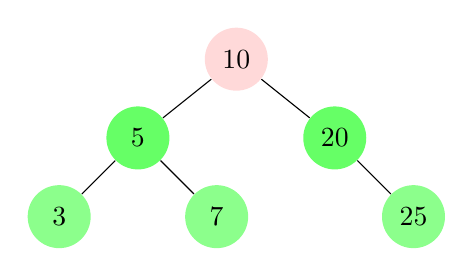
\begin{tikzpicture}[level distance=10mm]
        \tikzstyle{every node}=[fill=green!75,circle,inner sep=1pt, minimum size=8mm]
        \tikzstyle{level 1}=[sibling distance=25mm, set style={{every node}+=[fill=green!60]}]
        \tikzstyle{level 2}=[sibling distance=20mm, set style={{every node}+=[fill=green!45]}]
        \tikzstyle{level 3}=[sibling distance=15mm, set style={{every node}+=[fill=green!30]}]
        \tikzstyle{level 4}=[sibling distance=10mm, set style={{every node}+=[fill=green!15]}]
        \node[fill=pink!60] {10} child {node {5} child {node {3} } child {node {7} }} child {node {20} child[fill=none] {edge from parent[draw=none]} child {node {25} }};
    \end{tikzpicture}
    \caption{Initial Tree State}
\end{minipage}
\vspace{1cm}
\end{figure}

% Traversal Steps
\section*{Traversal Steps}
The following figures depict the binary tree as it is traversed using the selected traversal method. Each step highlights the node currently being processed.


\begin{figure}[h!]
\centering

\begin{minipage}{0.8\textwidth}
    \centering
    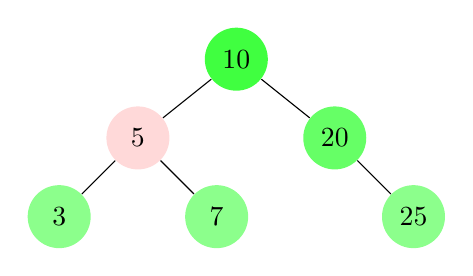
\begin{tikzpicture}[level distance=10mm]
        \tikzstyle{every node}=[fill=green!75,circle,inner sep=1pt, minimum size=8mm]
        \tikzstyle{level 1}=[sibling distance=25mm, set style={{every node}+=[fill=green!60]}]
        \tikzstyle{level 2}=[sibling distance=20mm, set style={{every node}+=[fill=green!45]}]
        \tikzstyle{level 3}=[sibling distance=15mm, set style={{every node}+=[fill=green!30]}]
        \tikzstyle{level 4}=[sibling distance=10mm, set style={{every node}+=[fill=green!15]}]
        \node {10} child {node[fill=pink!60] {5} child {node {3} } child {node {7} }} child {node {20} child[fill=none] {edge from parent[draw=none]} child {node {25} }};
    \end{tikzpicture}
    \caption{Step 2}
\end{minipage}
\vspace{1cm}

\begin{minipage}{0.8\textwidth}
    \centering
    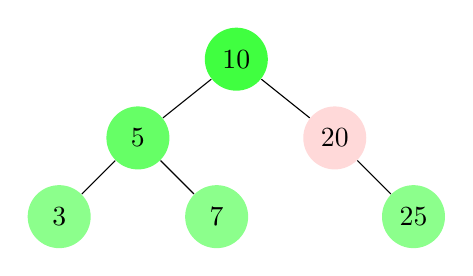
\begin{tikzpicture}[level distance=10mm]
        \tikzstyle{every node}=[fill=green!75,circle,inner sep=1pt, minimum size=8mm]
        \tikzstyle{level 1}=[sibling distance=25mm, set style={{every node}+=[fill=green!60]}]
        \tikzstyle{level 2}=[sibling distance=20mm, set style={{every node}+=[fill=green!45]}]
        \tikzstyle{level 3}=[sibling distance=15mm, set style={{every node}+=[fill=green!30]}]
        \tikzstyle{level 4}=[sibling distance=10mm, set style={{every node}+=[fill=green!15]}]
        \node {10} child {node {5} child {node {3} } child {node {7} }} child {node[fill=pink!60] {20} child[fill=none] {edge from parent[draw=none]} child {node {25} }};
    \end{tikzpicture}
    \caption{Step 3}
\end{minipage}
\vspace{1cm}

\begin{minipage}{0.8\textwidth}
    \centering
    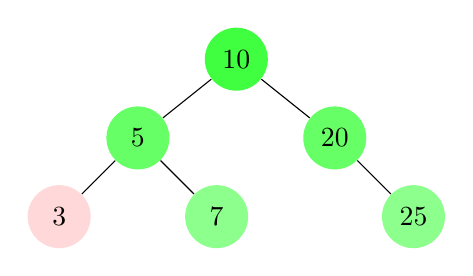
\begin{tikzpicture}[level distance=10mm]
        \tikzstyle{every node}=[fill=green!75,circle,inner sep=1pt, minimum size=8mm]
        \tikzstyle{level 1}=[sibling distance=25mm, set style={{every node}+=[fill=green!60]}]
        \tikzstyle{level 2}=[sibling distance=20mm, set style={{every node}+=[fill=green!45]}]
        \tikzstyle{level 3}=[sibling distance=15mm, set style={{every node}+=[fill=green!30]}]
        \tikzstyle{level 4}=[sibling distance=10mm, set style={{every node}+=[fill=green!15]}]
        \node {10} child {node {5} child {node[fill=pink!60] {3} } child {node {7} }} child {node {20} child[fill=none] {edge from parent[draw=none]} child {node {25} }};
    \end{tikzpicture}
    \caption{Step 4}
\end{minipage}
\vspace{1cm}

\begin{minipage}{0.8\textwidth}
    \centering
    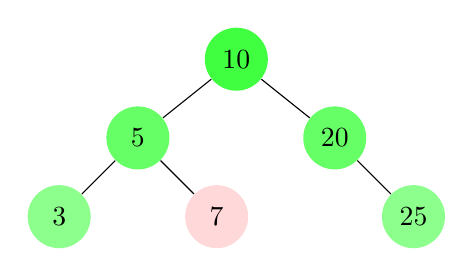
\begin{tikzpicture}[level distance=10mm]
        \tikzstyle{every node}=[fill=green!75,circle,inner sep=1pt, minimum size=8mm]
        \tikzstyle{level 1}=[sibling distance=25mm, set style={{every node}+=[fill=green!60]}]
        \tikzstyle{level 2}=[sibling distance=20mm, set style={{every node}+=[fill=green!45]}]
        \tikzstyle{level 3}=[sibling distance=15mm, set style={{every node}+=[fill=green!30]}]
        \tikzstyle{level 4}=[sibling distance=10mm, set style={{every node}+=[fill=green!15]}]
        \node {10} child {node {5} child {node {3} } child {node[fill=pink!60] {7} }} child {node {20} child[fill=none] {edge from parent[draw=none]} child {node {25} }};
    \end{tikzpicture}
    \caption{Step 5}
\end{minipage}
\vspace{1cm}

\begin{minipage}{0.8\textwidth}
    \centering
    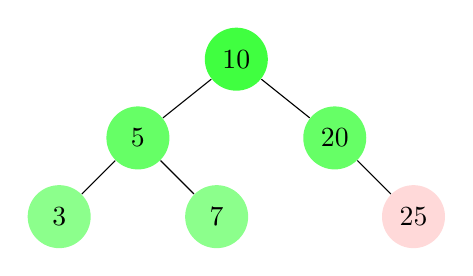
\begin{tikzpicture}[level distance=10mm]
        \tikzstyle{every node}=[fill=green!75,circle,inner sep=1pt, minimum size=8mm]
        \tikzstyle{level 1}=[sibling distance=25mm, set style={{every node}+=[fill=green!60]}]
        \tikzstyle{level 2}=[sibling distance=20mm, set style={{every node}+=[fill=green!45]}]
        \tikzstyle{level 3}=[sibling distance=15mm, set style={{every node}+=[fill=green!30]}]
        \tikzstyle{level 4}=[sibling distance=10mm, set style={{every node}+=[fill=green!15]}]
        \node {10} child {node {5} child {node {3} } child {node {7} }} child {node {20} child[fill=none] {edge from parent[draw=none]} child {node[fill=pink!60] {25} }};
    \end{tikzpicture}
    \caption{Step 6}
\end{minipage}
\vspace{1cm}

\end{figure}
\newpage

\end{document}
